\documentclass[10pt,twocolumn,letterpaper]{article}

\usepackage{cvpr}
\usepackage{times}
\usepackage{epsfig}
\usepackage{graphicx}
\usepackage{amsmath}
\usepackage{amssymb}

% Include other packages here, before hyperref.

% If you comment hyperref and then uncomment it, you should delete
% egpaper.aux before re-running latex.  (Or just hit 'q' on the first latex
% run, let it finish, and you should be clear).
%\usepackage[pagebackref=true,breaklinks=true,letterpaper=true,colorlinks,bookmarks=false]{hyperref}

\cvprfinalcopy % *** Uncomment this line for the final submission

\def\cvprPaperID{1} % *** Enter the CVPR Paper ID here
\def\httilde{\mbox{\tt\raisebox{-.5ex}{\symbol{126}}}}

% Pages are numbered in submission mode, and unnumbered in camera-ready
\ifcvprfinal\pagestyle{empty}\fi
\begin{document}

%%%%%%%%% TITLE
\title{ Program 2: Fun with Homographies}

\author{Brian Fehrman\\
SDSM\&T\\
501 E. Saint Joseph Street\\
{\tt\small bcfehrman@gmai1.com}
\thispagestyle{empty}
}

\maketitle
%%%%%%%%% ABSTRACT
\begin{abstract}
In this work I explored feature detection, extraction/description, and matching. The method implemented was a version of the Harris-Laplace method which offers scale, rotation, and illumination invariance when properly implemented. In addition to this, adaptive non-maximum suppression was also implemented and found to have better results than just picking the features with the largest response. A special pruning algorithm has also been implemented during the matching stage which will not allow for multiple matches to the same point and instead will pick the best pair of matches. This pruning along with using the ratio test (instead of just the SSD) was found to get rid of a large amount of the false matches that were present before implementing these techniques. All bench mark images were tested using the same tuning variable values such as the smoothing/derivation scales and the thresholds. Lastly, the algorithm was extended to work on live video feed and is able to track features between successive frames quite well.

\end{abstract}

%%%%%%%%% BODY TEXT


\section{Introduction}
The main purpose of this project was to get an introduction to working with homographies in order to perform perspective transforms from one image to another. Four applications of a homography have been rolled in to one program: transforming an entire picture in to chosen frame within another image (semi-auto frame stitching), transforming an arbitrary quadrilateral area from one image into an arbitrary frame within another image (manual frame stitching), manual choosing correspondence points in two images to create a mosaic (manual mosaic stitching), and having correspondence points chosen automatically from two images in order to create a mosaic. Each of these applications will be discussed further within this paper. The program was written using OpenCV with C++. The main references were Dr. Randy Hoover's slides as well as Dr. Szeliski's book.

%----------------------------1---------------------------------------------
\section{Start-Up}

At program start up the user is given a menu of choices for which homography application he or she would like to use (Figure \ref{fig:menu}). The program expects two images as inputs and can accept a wide variety of image formats.

\begin{figure*}[ht!]
\centering
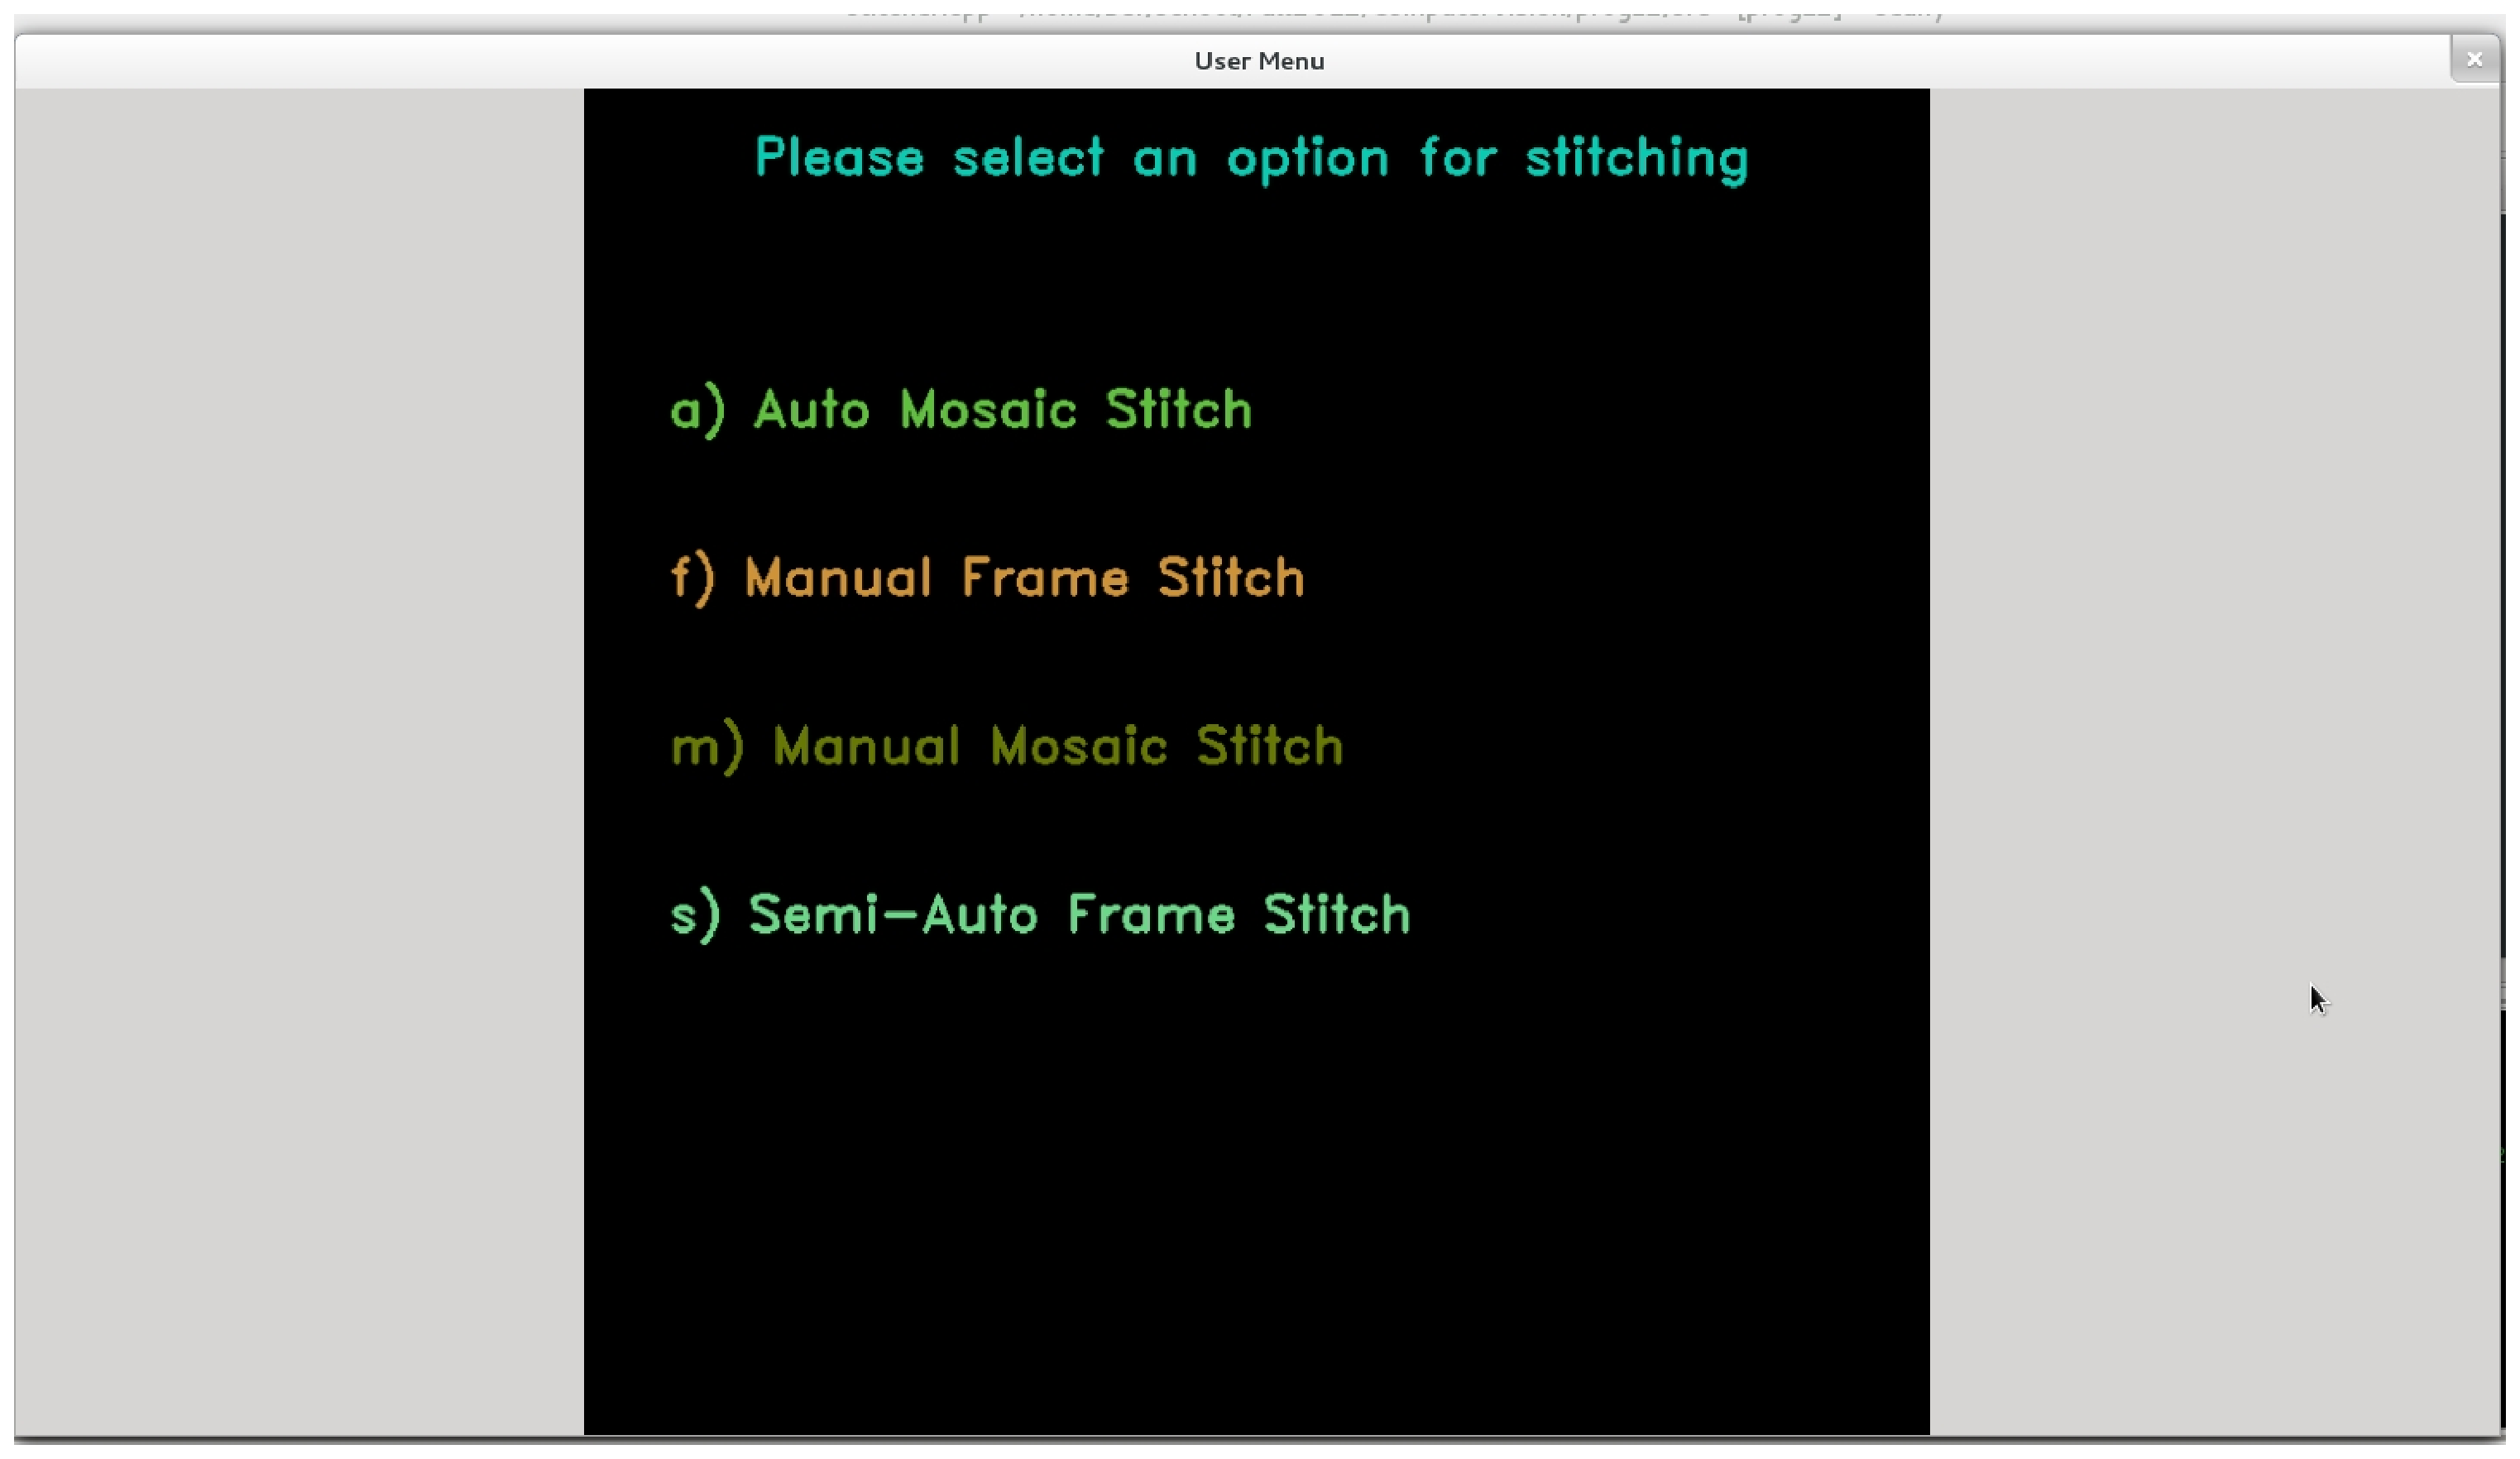
\includegraphics[width=0.6\textwidth]{img/prog_2_menu.eps}
\caption{Simple start up menu for Program 2}
\label{fig:menu}
\end{figure*}

\section{ Manual Frame Stitch }
Manual frame stitch is the feature that allows the user to select four points from one image (\emph{p image}) to form an arbitrary quadrilateral. The user then selects four corresponding points from a second image (\emph{p prime image}) that is displayed side-by-side by with the first image (Figure \ref{fig:man_frame_points} ). The program the computes two homography matrix (H matrix) estimates in order to determine the transformation between the two quadrilaterals. Each H matrix is computed using OpenCV's SVD routine to find the null space of the A matrix that is constructed from the chosen bounding points. The first H matrix transforms a nicely shaped box in to the $p$ chosen shape. This idea was chosen to make it easier to retrieve only the points that lie within the shape formed by the chosen $p$ points. The shape of the box is chosen to the dimensions of the largest extremist among the points (i.e, longest x and y distance among the chosen points). The idea for choosing a larger sized box was that less information would be lost in the transformation. It is quite possible that a box of any large size could be chosen for this. Using the transformation from the box to $p$, then each pixel in the box is iterated through and transformed in order to determine from where in the \emph{p image} the current pixel should be taken. Once the box's pixels have been populated with pixels from within the area enclosed by the $p$ points then those pixels are transformed using the box to $p'$ H matrix. As before, each pixel in the box is iterated through but this time the H matrix transformation is used to determine where each of the box's pixels will be placed within the shape formed by the $p'$ points.

\begin{figure*}[ht!]
\centering
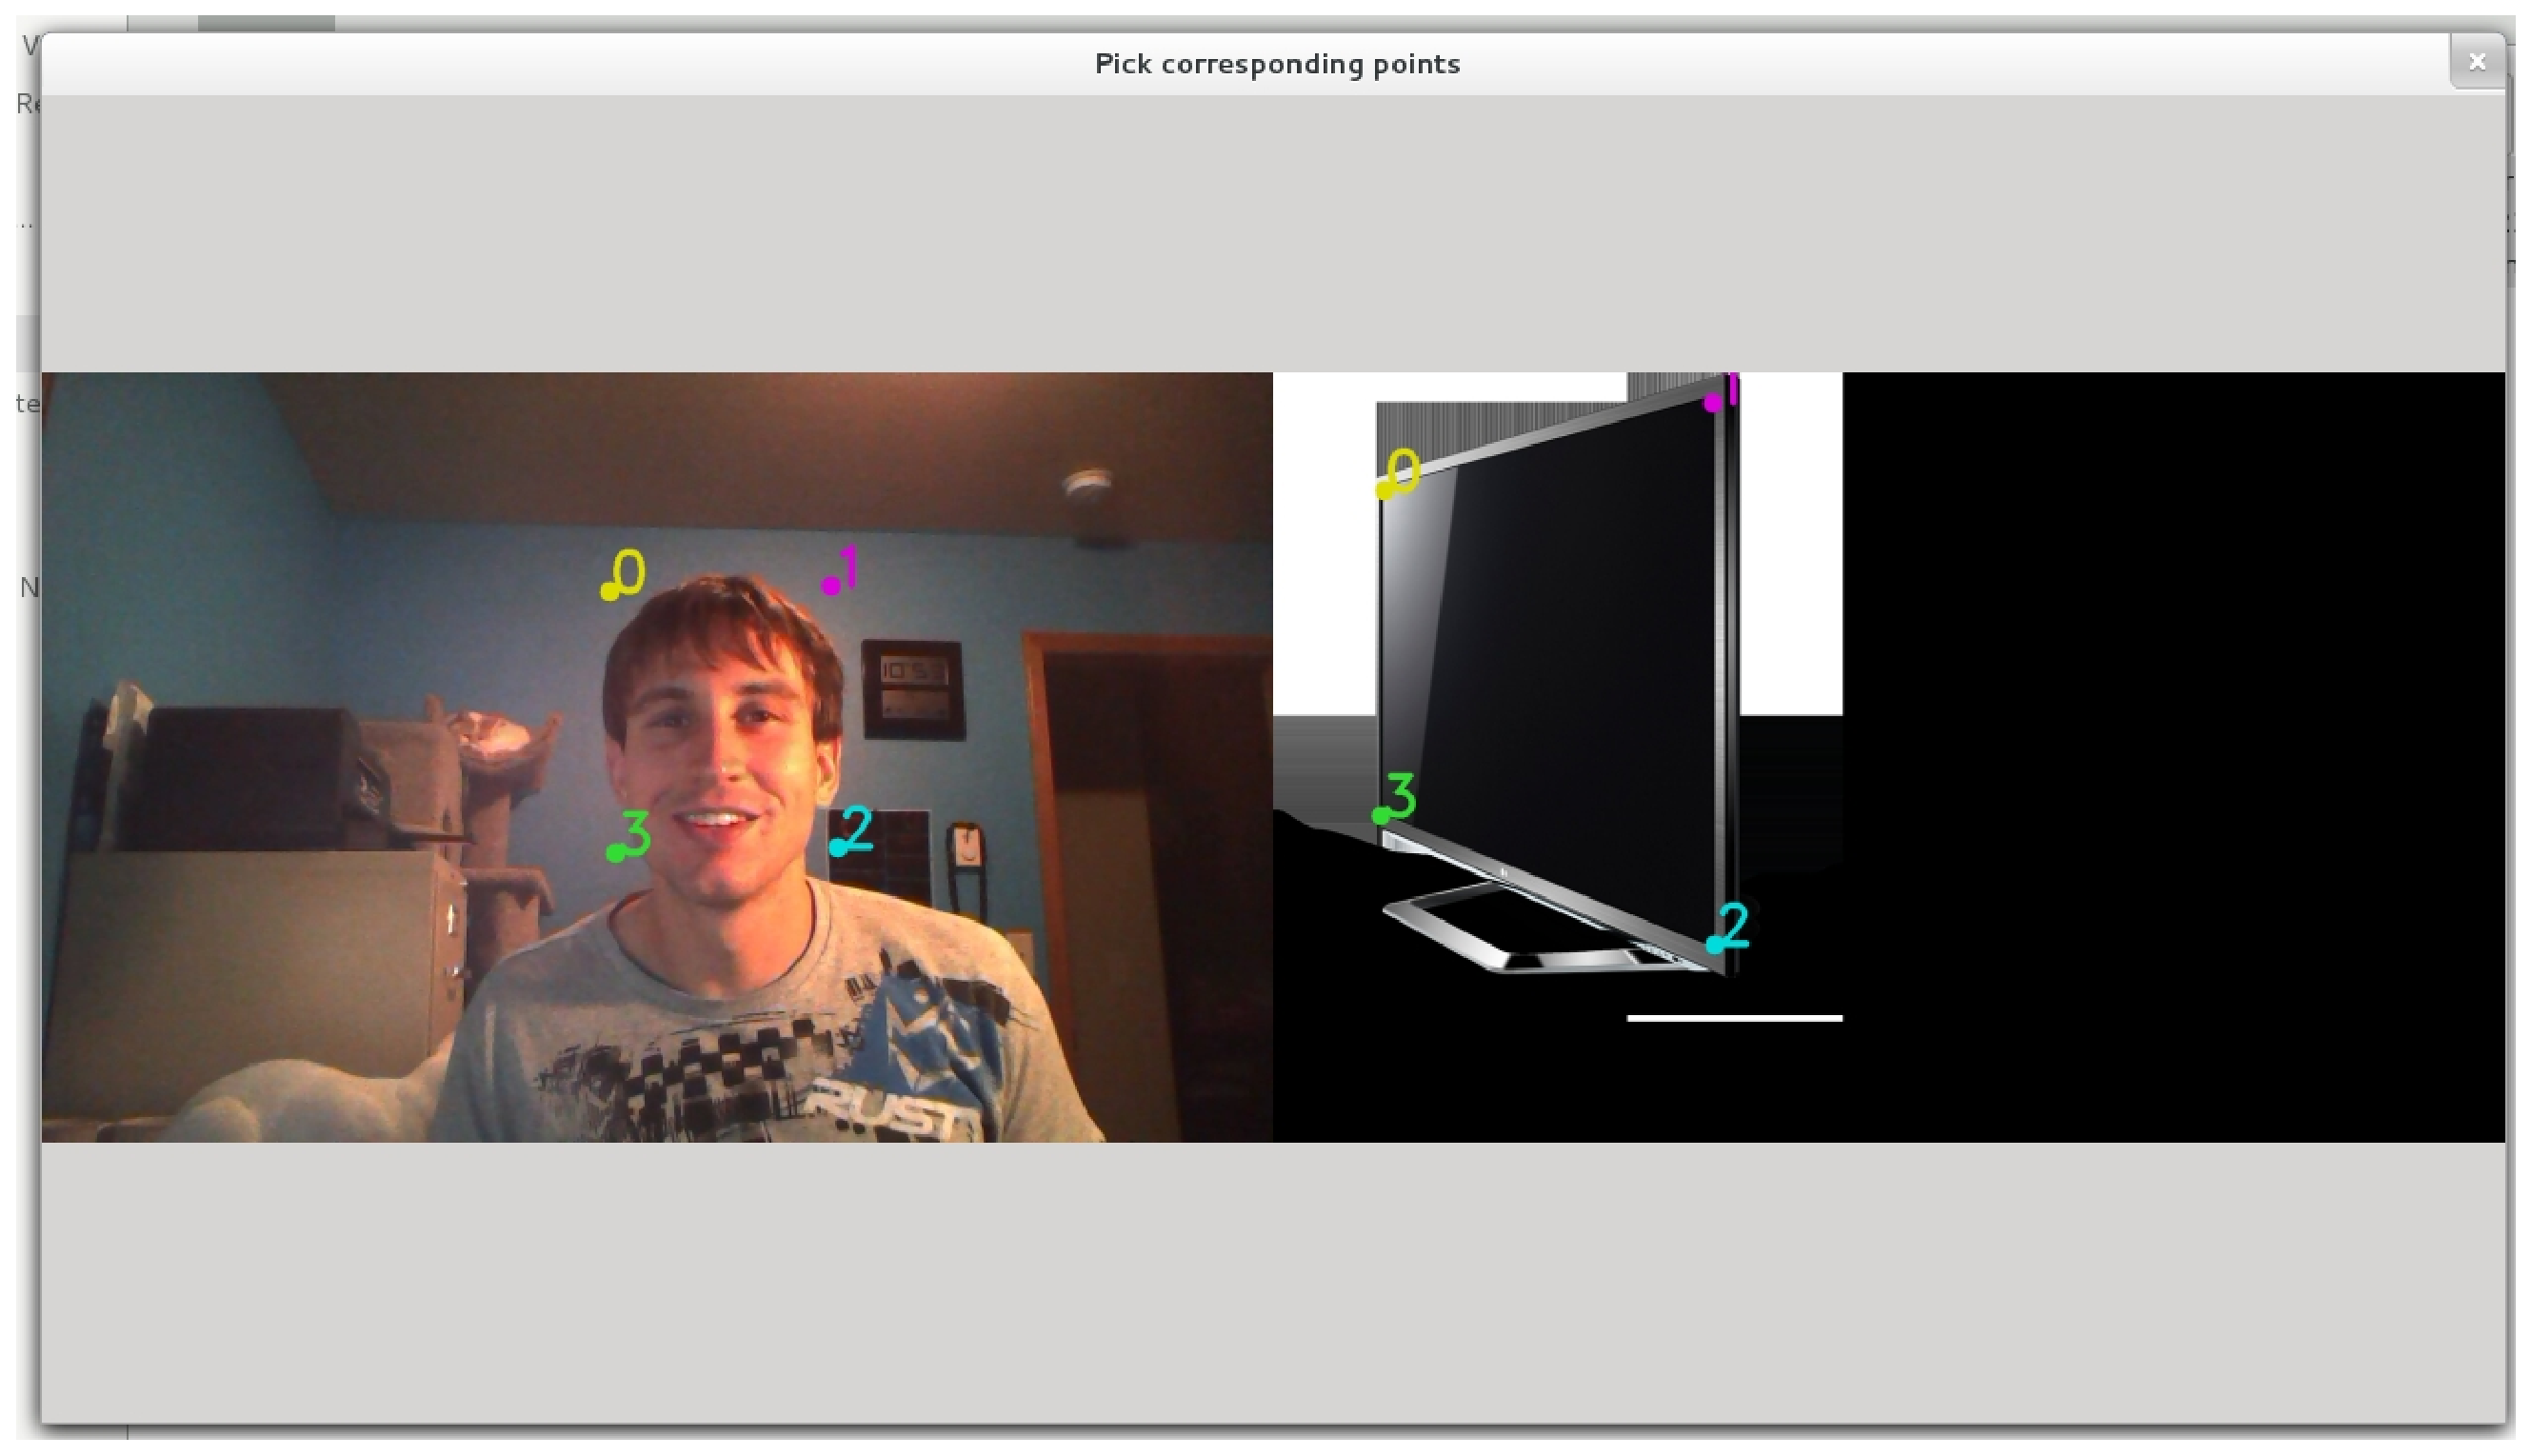
\includegraphics[width=0.6\textwidth]{img/man_frame_points.eps}
\caption{Selection of four correspondence points in each image. The image on the image on the left is $p$ and the image on the right is $p'$.}
\label{fig:man_frame_points}
\end{figure*}


\section{ Semi-Automatic Frame Stitch }
The semi-automatic frame stitch is very similar to the manual frame stitch. However, instead of the user selecting four points from the \emph{p image} the program uses the four corners of the $p image$ as the reference for transformation so that the entire image will be warped in to a new frame in the \emph{ p prime image}. The user still selects four points in the \emph{p prime image} to construct the frame in to which the \emph{p image} will be transformed (Figure \ref{fig:semi_auto_frame_points} ). The same procedure as the manual frame stitching algorithm is used for computing the two H matrices and using them to transform the points. 

\begin{figure*}[ht!]
\centering
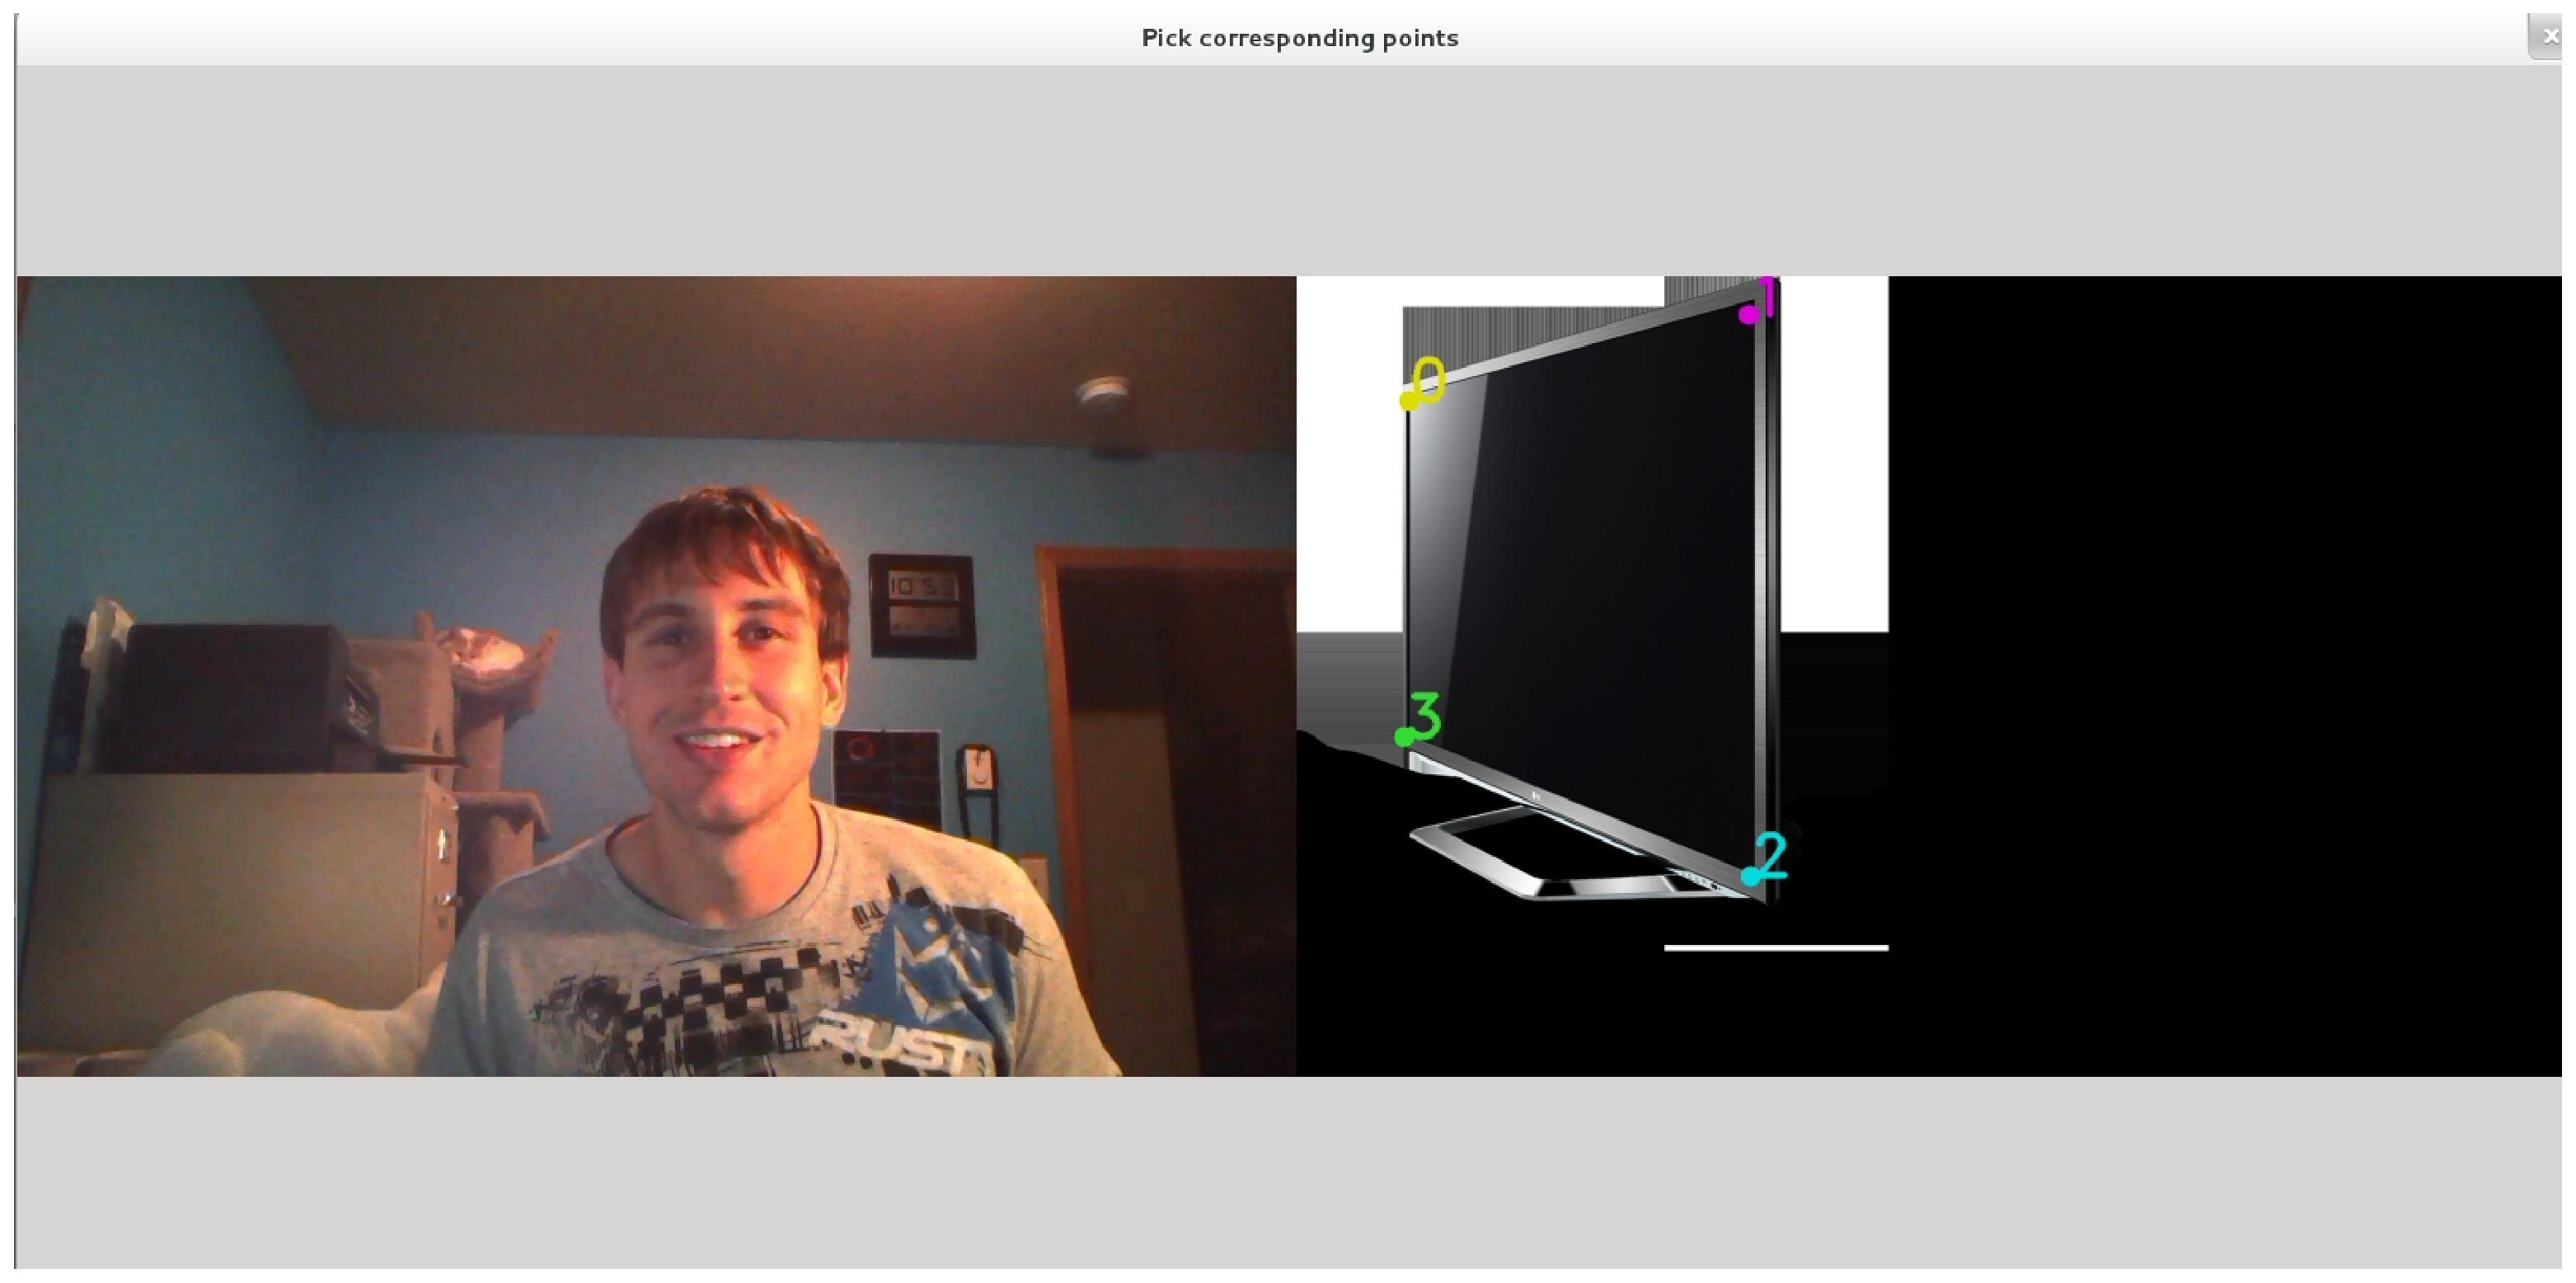
\includegraphics[width=0.6\textwidth]{img/semi_auto_frame_points.eps}
\caption{Selection of four correspondence points in just the \emph{p prime image}. The four corners of the \emph{p image} are used for the semi-automatic frame stitching instead of letting the user select four points from that image.}
\label{fig:semi_auto_frame_points}
\end{figure*}


\section{Manual Mosaic Stitch}
For the manual mosaic stitch the initial procedure is largely the same as that for the manual frame stitching. The user selects four correspondence points from two side by side images. The main difference in this case, however, is that the user to attempt to select points that actually do correspond to one another in terms of locating features that are common between the two images but are seen in different locations in each image (Figure \ref{fig:man_mosaic_points} ). If points are chosen which do not represent common features then the mosaic will not work correctly. Ones the points have been chosen then H matrix is computed which takes  the $p$ points directly to the $p'$ points. A new new output frame is created and its dimensions are chosen to accommodate the max $p'$ transformed points that are encountered when multiplying each $p'$ point by the inverse of the H matrix which takes $p'$ points to $p$ and was calculated using OpenCV's matrix inverse function. The $p$ points are copied verbatim to the new output frame (where the $p$ points were assumed to have come from the left hand image). All of the $p'$ points are transformed in to the output frame by using the inverse of the H matrix. Additionally, to fill in the black spaces, each the H matrix is applied to each pixel in the output frame to determine where from in the \emph{p prime image } to grab a pixel to fill the current pixel. Neither splattering nor interpolation techniques were used without drastically dire consequences.

\begin{figure*}[ht!]
\centering
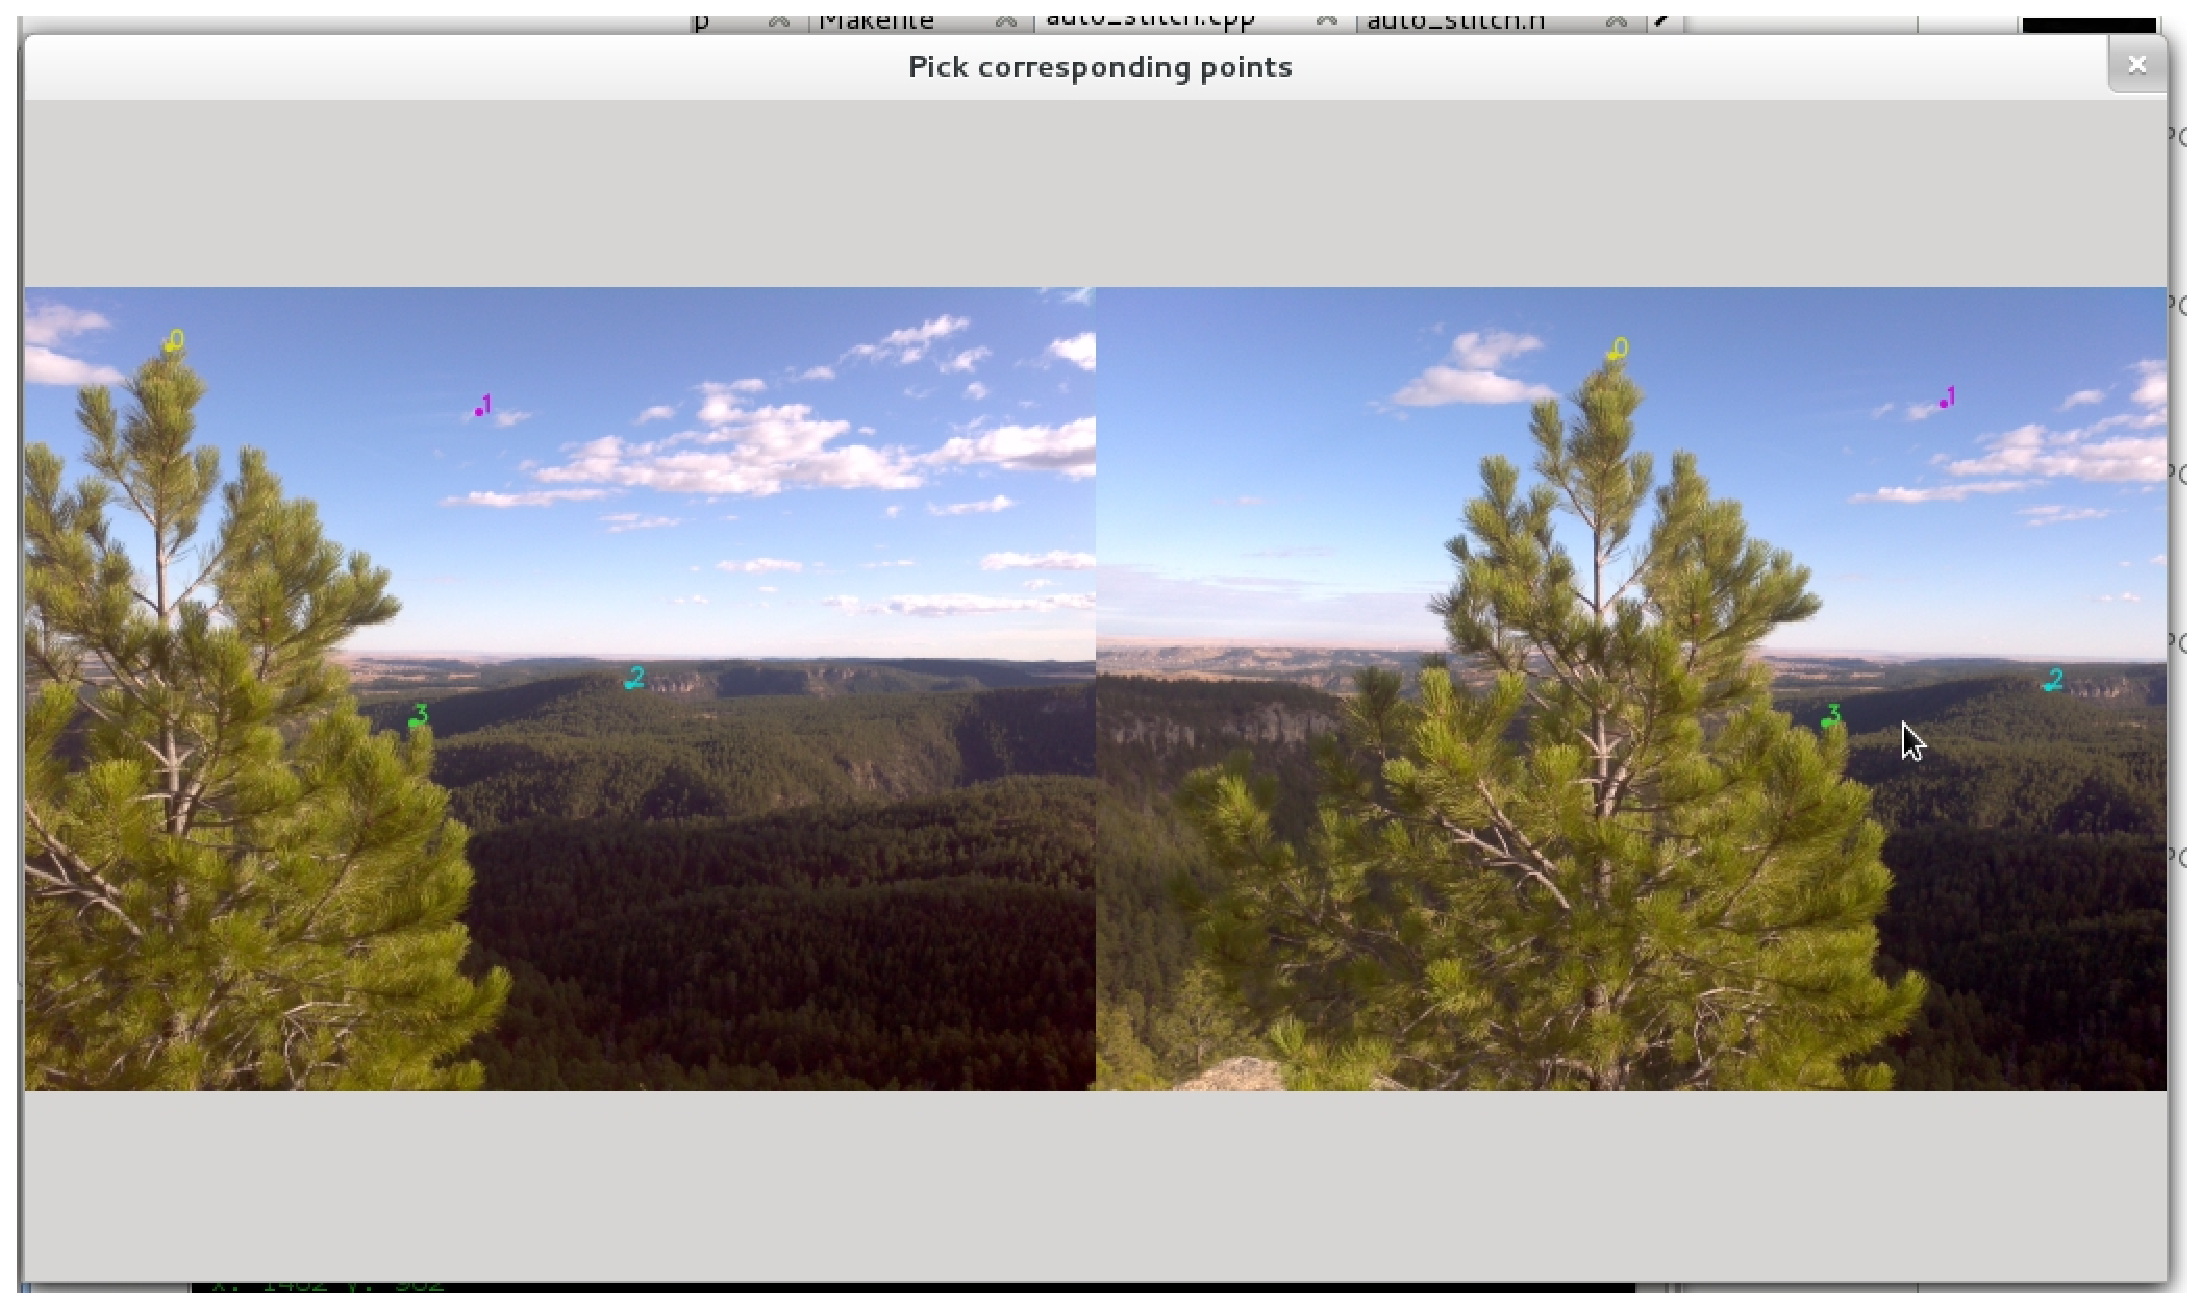
\includegraphics[width=0.6\textwidth]{img/manual_mosaic_points.eps}
\caption{Selection of four correspondence points in each image that were used for manual mosaic stitching.}
\label{fig:man_mosaic_points}
\end{figure*}
{\small
\bibliographystyle{ieee}
\bibliography{egbib}
}

\section{Automatic Mosaic Stitching}
The automatic mosaic stitching was just a matter of automatically obtaining matching correspondence points from two input images rather than letting the user select those points as with the manual mosaic stitching. OpenCV's SURF detect function was used to find key points in each image and were placed in to a vector of \emph{KeyPoint} structs. I then ran my own adaptive non-maximum suppression algorithm on the SURF key points in order to find local maxima that were 10\% greater in value than any neighbors within a five pixel radius. This also forced the points to have at least a reasonable spacing among themselves. The feature descriptions were then extracted at each remaining key point by the use of OpenCV's SURF extract function. The features were then matched using OpenCV's FLANN matching function which places potential matches into a vector of \emph{DMatch} structs. The matches are then sorted by ascending distance and the top 50 matches are kept. My self-implemented RANSAC algorithm is then performed on the 50 remaining points in order to further ensure that good matches are being used to form the H matrix. 10 points are selected at random from the 50 potential matches. There is logic in place to ensure that the same point is not selected twice. H is then computed for the given set of random points and is then applied to all $p$ match points which are then compared to all of the $p'$ match points. A tally is kept of how many potential match points the current H matrix successfully transforms and this information is used to select the best H matrix. The $p$ and $p'$ points are then transferred to the output frame using the same procedure as was used for the manual mosaic stitching.

\end{document}
